% ==========================================================================
%  SPHERExLens -- A0 conference poster (portrait, 841 x 1189 mm)
%  Build:  pdflatex spherexlens_poster.tex
% ==========================================================================
\documentclass[10pt]{article}

\usepackage[T1]{fontenc}
\usepackage[utf8]{inputenc}
\usepackage{lmodern}
\usepackage[paperwidth=841mm,paperheight=1189mm,margin=14mm]{geometry}
\usepackage{amsmath,amssymb}
\usepackage{xcolor}
\usepackage{tikz}
\usetikzlibrary{arrows.meta,positioning,calc,fit,backgrounds}
\usepackage{pgfplots}
\pgfplotsset{compat=1.18}
\usepackage{booktabs,array}
\usepackage{enumitem}
\usepackage[most]{tcolorbox}

% ------------------------------------------------------------------ colours
\definecolor{ink}{HTML}{14213A}
\definecolor{slate}{HTML}{3F4A5A}
\definecolor{muted}{HTML}{6E7A8A}
\definecolor{accent}{HTML}{1F6FB2}
\definecolor{accent2}{HTML}{E8F1F8}
\definecolor{good}{HTML}{1E7B4F}
\definecolor{good2}{HTML}{E7F3EC}
\definecolor{bad}{HTML}{B3261E}
\definecolor{bad2}{HTML}{FAECEA}
\definecolor{warn}{HTML}{8A5A00}
\definecolor{warn2}{HTML}{FBF3E2}
\definecolor{rule}{HTML}{D5DAE2}
\definecolor{paper}{HTML}{F8F5F2}

\pagecolor{paper}
\pagestyle{empty}
\setlength{\parindent}{0pt}
\setlength{\parskip}{0pt}
\setlength{\emergencystretch}{3em}

% ------------------------------------------------------------------- macros
\newcommand{\bodyfont}{\fontsize{27}{34}\selectfont}
\newcommand{\smallfont}{\fontsize{20}{26}\selectfont}
\newcommand{\tinyfont}{\fontsize{17}{22}\selectfont}
\newcommand{\arcsec}{\ensuremath{{}^{\prime\prime}}}
\newcommand{\arcmin}{\ensuremath{{}^{\prime}}}

\newcommand{\pblock}[2]{%
  {\color{accent}\rule{\linewidth}{2.2mm}}\par\vspace{3mm}%
  {\fontsize{42}{50}\selectfont\bfseries\color{ink}#1\par}%
  \vspace{3.4mm}{\bodyfont\color{ink}#2\par}\vspace{34mm}}

\newcommand{\kpi}[3]{%
  \begin{tcolorbox}[enhanced jigsaw,colback=#1!9!white,colframe=#1!35!white,
    boxrule=0.5pt,arc=2mm,left=4mm,right=4mm,top=2.6mm,bottom=2.6mm,
    halign=center,valign=center]
    {\fontsize{34}{38}\selectfont\bfseries\color{#1}#2\par}
    \vspace{1mm}{\smallfont\color{ink}#3\par}
  \end{tcolorbox}}

\newenvironment{plist}{%
  \begin{itemize}[leftmargin=7mm,itemsep=2.2mm,topsep=1mm,label={\color{accent}\textbullet}]
  \bodyfont}{\end{itemize}}

\newcommand{\hi}[1]{{\color{accent}\textbf{#1}}}
\newcommand{\gx}[1]{{\color{good}\textbf{#1}}}
\newcommand{\bx}[1]{{\color{bad}\textbf{#1}}}

\begin{document}

% ================================================================ HEADER ==
\begin{tikzpicture}[remember picture,overlay]
  \fill[ink] (current page.north west) rectangle ([yshift=-96mm]current page.north east);
\end{tikzpicture}

\vspace*{0mm}
{\color{white!80!ink}\fontsize{16}{20}\selectfont\bfseries
  SPHEREX DATA RELEASE 1 \;\textbullet\; DIFFERENCE IMAGING \;\textbullet\; TRANSIENT DISCOVERY}
\par\vspace{5mm}
{\color{white}\fontsize{56}{62}\selectfont\bfseries Finding What Changed\par}
\vspace{3mm}
{\color{white!84!ink}\fontsize{27}{33}\selectfont
  An open, calibrated difference-imaging and candidate-discovery pipeline
  for the SPHEREx all-sky survey\par}
\vspace{4mm}
{\color{white!70!ink}\fontsize{19}{24}\selectfont
  Evan Lim \;\textbullet\; SPHERExLens collaboration \;\textbullet\; November 2026\par}
\vspace{7mm}

\noindent
\begin{minipage}[t]{0.238\linewidth}\kpi{accent}{18 / 246}{fields / cut-outs}\end{minipage}\hfill
\begin{minipage}[t]{0.238\linewidth}\kpi{warn}{109}{detections $\rightarrow$ 99 known, 10 candidates}\end{minipage}\hfill
\begin{minipage}[t]{0.238\linewidth}\kpi{good}{69.3\%}{strict injection recovery}\end{minipage}\hfill
\begin{minipage}[t]{0.238\linewidth}\kpi{bad}{1.66}{false candidates per field}\end{minipage}


% ============================================================== 3 COLUMNS ==
\noindent\makebox[\linewidth][l]{%
\begin{minipage}[t][0.76\textheight][t]{0.317\linewidth}

\vfill
\pblock{Why difference imaging}{%
A single image fixes position in time. A second visit, six months later, turns the same patch of sky
into a measurement of \emph{motion} and \emph{brightness}:
\begin{plist}
  \item subtract the visits and the stationary sky cancels;
  \item a \hi{dipole} is a source that moved;
  \item a \hi{monopole} is a source that brightened or faded.
\end{plist}
But the two visits never share a point-spread function. Instrumental residuals outnumber real events
by \bx{\(\sim\)1000\(\times\)}, so the task is not subtraction --- it is deciding which residuals are
astrophysics.}

\centering
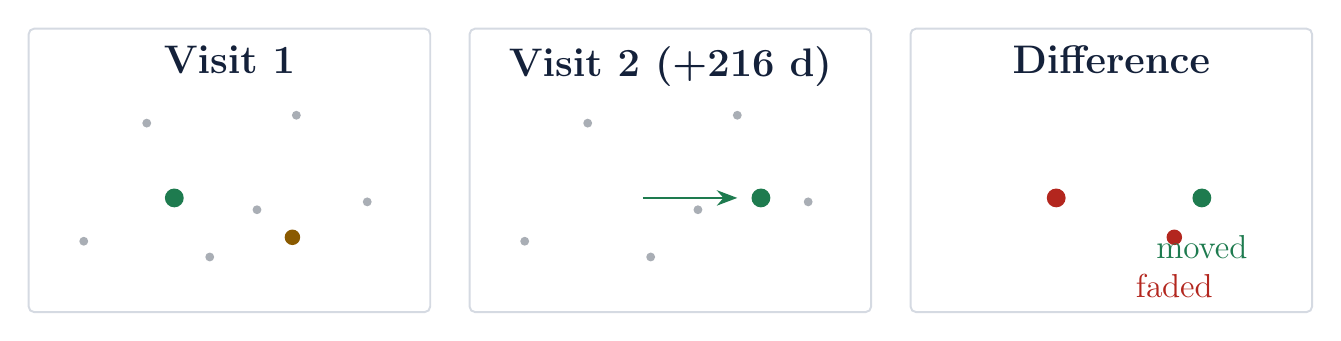
\begin{tikzpicture}[font=\fontsize{13}{16}\selectfont]
  \foreach \i/\lab in {0/{Visit 1},1/{Visit 2 (+216 d)},2/{Difference}}{
    \draw[rule,line width=0.7pt,fill=white,rounded corners=2pt]
      (\i*5.6,0) rectangle (\i*5.6+5.1,3.6);
    \node[text=ink,font=\fontsize{14}{17}\selectfont\bfseries,anchor=north]
      at (\i*5.6+2.55,3.5) {\lab};
  }
  \foreach \x/\y in {0.7/0.9,1.5/2.4,2.3/0.7,3.4/2.5,4.3/1.4,2.9/1.3}{
    \fill[slate!45] (\x,\y) circle (1.6pt);
    \fill[slate!45] (\x+5.6,\y) circle (1.6pt);
  }
  \fill[good] (1.85,1.45) circle (3.4pt);
  \fill[good] (5.6+3.7,1.45) circle (3.4pt);
  \draw[-{Stealth[length=2.6mm]},good,line width=0.9pt] (5.6+2.2,1.45) -- (5.6+3.4,1.45);
  \fill[warn] (3.35,0.95) circle (2.8pt);
  \fill[bad] (11.2+1.85,1.45) circle (3.4pt);
  \fill[good] (11.2+3.7,1.45) circle (3.4pt);
  \fill[bad] (11.2+3.35,0.95) circle (2.8pt);
  \node[text=good,font=\fontsize{13}{16}\selectfont,anchor=north] at (11.2+3.7,1.1) {moved};
  \node[text=bad,font=\fontsize{13}{16}\selectfont,anchor=north] at (11.2+3.35,0.6) {faded};
\end{tikzpicture}

\raggedright
\vspace{1mm}
{\tinyfont\color{slate}The stationary sky subtracts to zero; green = positive, red = negative.\par}

\vspace{6mm}
\vfill
\pblock{The task, stated}{%
Two \(180\times180\) pixel cut-outs, their variance planes and a 32-bit quality mask; one
significance map \(S\); a \(6.0\sigma\) threshold; \hi{109 detections}. Each detection must be given
an identity before it can be called a candidate:
\begin{plist}
  \item \gx{99 KNOWN} --- catalogue star, asteroid or optical artefact;
  \item \hi{10 CANDIDATE} --- unexplained by Gaia, AllWISE, NEOWISE or VSX.
\end{plist}
Constraints: public archive data only, every number reproducible, and \emph{``no change''} kept
strictly distinct from \emph{``no data''}.}

\vfill
\pblock{Where it sits}{%
\begin{plist}
  \item \textbf{1998} Alard \& Lupton --- kernel fitted from bright stars.
  \item \textbf{2008} Bramich --- discrete per-pixel kernel.
  \item \textbf{2016} ZOGY --- closed-form Fourier subtraction, analytic null.
  \item \textbf{2022} SFFT --- delta-basis kernels for undersampled space PSFs.
\end{plist}
Brokers (ANTARES, ALeRCE, Lasair, Fink) industrialise the veto for optical alerts, but they start
from alerts, not pixels. No open, end-to-end, inspectable pipeline existed for SPHEREx Level-2 data
--- \hi{that is the gap this work fills}.}

\end{minipage}\hfill

\begin{minipage}[t][0.76\textheight][t]{0.317\linewidth}

\vfill
\pblock{The data}{%
\begin{plist}
  \item \textbf{102 bands}, 0.75--5.0\,\textmu m, from a linear variable filter: every pixel has its
        own colour.
  \item \textbf{6 extensions} per cut-out: IMAGE, FLAGS (32-bit), VARIANCE, WCS-WAVE, EPSF, ZODI.
  \item \textbf{6-month cadence}: solar-system objects leave the field between visits.
  \item \textbf{18} fields, \textbf{246} cut-outs, fetched as \(\sim\)5\,MB stamps rather than
        70\,MB parent frames; each must keep a 12-px margin and \(<50\%\) flagged pixels.
\end{plist}}

\vfill
\pblock{Seven subsystems, one science core}{%
\centering
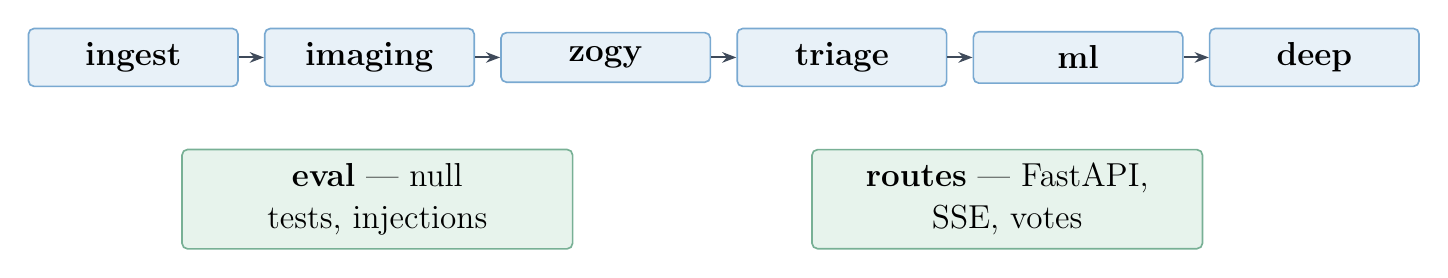
\begin{tikzpicture}[font=\fontsize{12}{15}\selectfont,
  b/.style={draw=accent!60,fill=accent2,line width=0.6pt,rounded corners=2pt,
    align=center,inner sep=1.8mm},
  ar/.style={-{Stealth[length=1.8mm]},draw=slate,line width=0.7pt}]
  \node[b,text width=23mm] (i) at (0.9,2.9) {\textbf{ingest}};
  \node[b,text width=23mm] (m) at (3.9,2.9) {\textbf{imaging}};
  \node[b,text width=23mm] (z) at (6.9,2.9) {\textbf{zogy}};
  \node[b,text width=23mm] (t) at (9.9,2.9) {\textbf{triage}};
  \node[b,text width=23mm] (l) at (12.9,2.9) {\textbf{ml}};
  \node[b,text width=23mm] (d) at (15.9,2.9) {\textbf{deep}};
  \draw[ar] (i)--(m); \draw[ar] (m)--(z); \draw[ar] (z)--(t); \draw[ar] (t)--(l); \draw[ar] (l)--(d);
  \node[draw=good!60,fill=good2,line width=0.6pt,rounded corners=2pt,align=center,inner sep=1.8mm,
    text width=46mm] (e) at (4.0,1.1) {\textbf{eval} --- null tests, injections};
  \node[draw=good!60,fill=good2,line width=0.6pt,rounded corners=2pt,align=center,inner sep=1.8mm,
    text width=46mm] (r) at (12.0,1.1) {\textbf{routes} --- FastAPI, SSE, votes};
\end{tikzpicture}

\raggedright
\vspace{1mm}
{\tinyfont\color{slate}One JSON contract; 21\,429 runtime Python lines; identical results in batch and
in the live service.\par}}

\vspace{6mm}
\vfill
\pblock{Method: proper subtraction}{%
ZOGY convolves each image with the \emph{other} image's point-spread function and divides by the
surviving noise --- nothing is fitted:
\[
  \hat D=\frac{\hat P_1\hat I_2-\hat P_2\hat I_1}
                {\sqrt{\sigma_1^2|\hat P_2|^2+\sigma_2^2|\hat P_1|^2}},
  \qquad
  S=\frac{\hat D\,\hat P_D}{\sqrt{\hat\sigma_1^2+\hat\sigma_2^2}} .
\]
The significance map is \hi{unit-variance Gaussian} wherever the sky is constant, so the threshold
is a probability statement rather than a tuning knob. Cost: two 2-D FFTs per epoch pair, \(<0.6\)\,s
for a \(180^2\) frame. Empirical PSFs come from a \(21\times21\) detector-zone grid chosen through the
cut-out's WCS.}

\vfill
\pblock{Detection statistics}{%
\centering
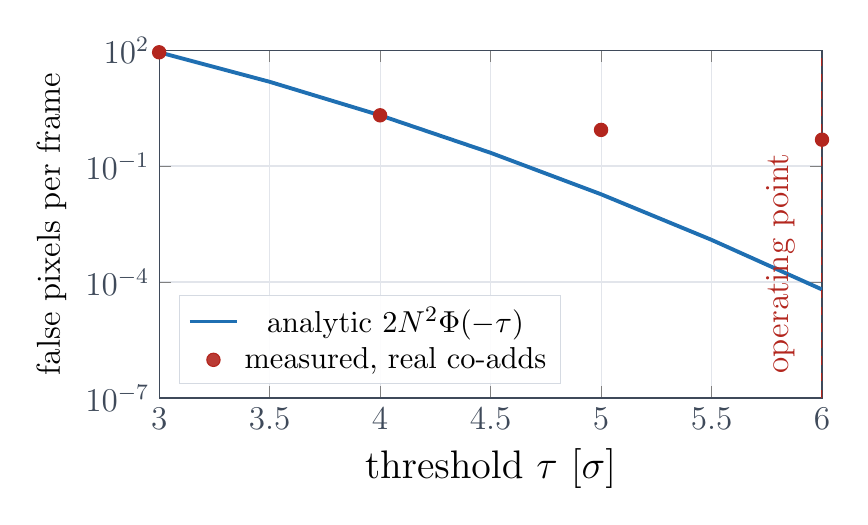
\begin{tikzpicture}[font=\fontsize{13}{16}\selectfont]
  \begin{axis}[width=100mm,height=60mm,xmin=3,xmax=6,ymin=1e-7,ymax=1e2,ymode=log,
    xlabel={threshold \(\tau\) [\(\sigma\)]},ylabel={false pixels per frame},
    xlabel style={font=\fontsize{14}{17}\selectfont},
    ylabel style={font=\fontsize{13}{16}\selectfont},
    tick label style={font=\fontsize{12}{15}\selectfont,text=slate},
    axis line style={slate},grid=major,grid style={rule!70},
    legend style={font=\fontsize{11}{14}\selectfont,draw=rule,at={(0.03,0.04)},anchor=south west,
      fill=white,fill opacity=0.9,text opacity=1}]
    \addplot[accent,line width=1.4pt] coordinates
      {(3,87.5) (3.5,15.1) (4,2.05) (4.5,0.220) (5,0.0186) (5.5,0.00123) (6,6.4e-5)};
    \addlegendentry{analytic \(2N^2\Phi(-\tau)\)}
    \addplot[only marks,mark=*,mark size=2.4pt,bad] coordinates
      {(3,87.5) (4,2.05) (5,0.86) (6,0.48)};
    \addlegendentry{measured, real co-adds}
    \draw[bad,dashed,line width=1.1pt] (axis cs:6,1e-7) -- (axis cs:6,1e2);
    \node[text=bad,font=\fontsize{12}{15}\selectfont,rotate=90,anchor=south]
      at (axis cs:5.92,3e-4) {operating point};
  \end{axis}
\end{tikzpicture}

\raggedright
\vspace{1mm}
{\tinyfont\color{slate}At \(5\sigma\) the Gaussian budget is 0.0186 per frame; the data give 0.86 per
field. At \(6\sigma\): 0.48, with no loss of strict recovery.\par}}

\end{minipage}\hfill

\begin{minipage}[t][0.76\textheight][t]{0.317\linewidth}

\vfill
\pblock{Results}{%
\centering
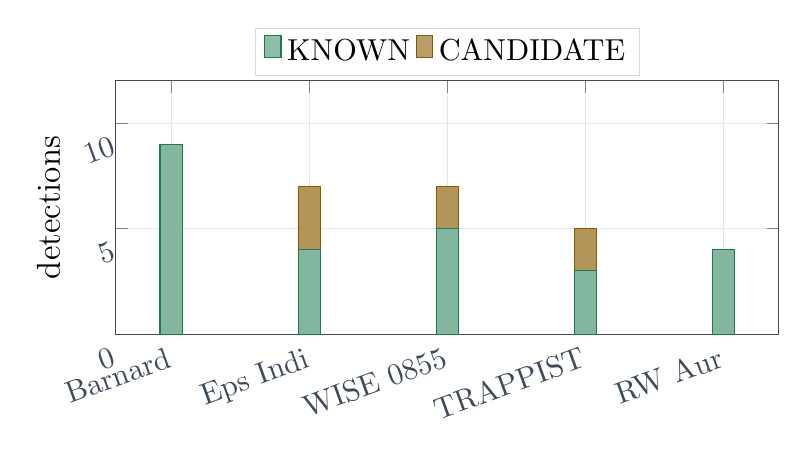
\begin{tikzpicture}[font=\fontsize{12}{15}\selectfont]
  \begin{axis}[width=100mm,height=48mm,ybar stacked,bar width=8pt,ymin=0,ymax=12,
    ylabel={detections},ylabel style={font=\fontsize{13}{16}\selectfont},
    symbolic x coords={{Barnard},{Eps Indi},{WISE 0855},{TRAPPIST},{RW Aur}},
    xtick=data,tick label style={font=\fontsize{11}{14}\selectfont,text=slate,rotate=20,
      anchor=north east},
    axis line style={slate},grid=major,grid style={rule!70},
    legend style={font=\fontsize{11}{14}\selectfont,draw=rule,at={(0.5,1.02)},anchor=south,
      legend columns=2,fill=white,fill opacity=0.9,text opacity=1}]
    \addplot[fill=good!55,draw=good] coordinates
      {({Barnard},9) ({Eps Indi},4) ({WISE 0855},5) ({TRAPPIST},3) ({RW Aur},4)};
    \addlegendentry{KNOWN}
    \addplot[fill=warn!65,draw=warn] coordinates
      {({Barnard},0) ({Eps Indi},3) ({WISE 0855},2) ({TRAPPIST},2) ({RW Aur},0)};
    \addlegendentry{CANDIDATE}
  \end{axis}
\end{tikzpicture}

\raggedright
\vspace{2mm}
{\bodyfont \hi{109} detections across 18 fields: \gx{99 KNOWN} (91\%), \hi{10 CANDIDATE} (9\%).
Detection count is not discovery count. Two fields return nothing --- Orion M42 is a null sky, and
Sgr\,A* is refused because the two epochs share no detector band.\par}

\vspace{3mm}
{\smallfont\color{ink}
\textbf{The ten candidates} sit in five fields: \(\epsilon\) Indi B (3), WISE 0855 (2), M45 (2),
TRAPPIST-1 (2), 3C 273 (1). All are faint infrared excesses beyond the Gaia and WISE limits ---
exactly what needs follow-up before anyone says \emph{discovery}.\par}

\vspace{3mm}
{\smallfont\color{slate}
Barnard's Star --- our first ``candidate'' --- was a coordinate-frame bug: 94\arcsec\ of proper motion
over 9.8\,yr. Propagating the Gaia position to the exposure epoch turns the 36.2\(\sigma\) dipole into
KNOWN\_MOVER and leaves \gx{zero} candidates in that field.\par}}

\vfill
\pblock{Validation}{%
\centering
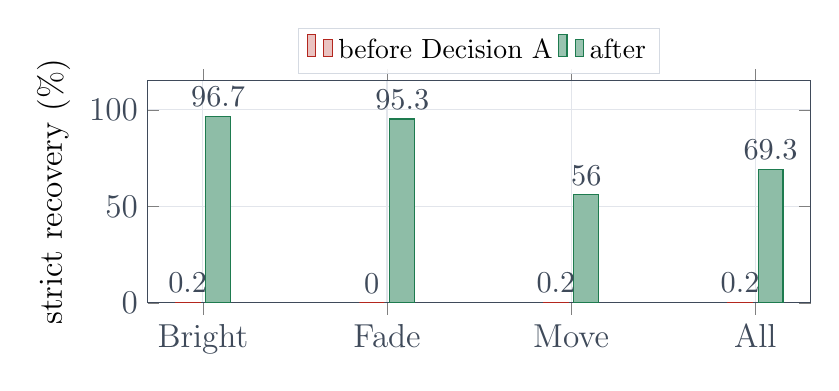
\begin{tikzpicture}[font=\fontsize{12}{15}\selectfont]
  \begin{axis}[width=100mm,height=44mm,ybar,bar width=9pt,ymin=0,ymax=115,
    ylabel={strict recovery (\%)},ylabel style={font=\fontsize{13}{16}\selectfont},
    symbolic x coords={{Bright},{Fade},{Move},{All}},
    xtick=data,tick label style={font=\fontsize{12}{15}\selectfont,text=slate},
    axis line style={slate},grid=major,grid style={rule!70},
    nodes near coords,nodes near coords style={font=\fontsize{11}{13}\selectfont\bfseries,text=slate},
    legend style={font=\fontsize{10}{13}\selectfont,draw=rule,at={(0.5,1.03)},anchor=south,
      legend columns=2,fill=white,fill opacity=0.9,text opacity=1}]
    \addplot[fill=bad!30,draw=bad] coordinates {({Bright},0.2) ({Fade},0) ({Move},0.2) ({All},0.2)};
    \addlegendentry{before Decision A}
    \addplot[fill=good!50,draw=good] coordinates
      {({Bright},96.7) ({Fade},95.3) ({Move},56.0) ({All},69.3)};
    \addlegendentry{after}
  \end{axis}
\end{tikzpicture}

\raggedright
\vspace{2mm}
\begin{plist}
  \item \textbf{Split-epoch null test.} 220 realisations, 17 fields, 3.57\,deg\(^2\): 8\,854 raw peaks
        \(\rightarrow\) \hi{1.66 false candidates per field}, \gx{zero in six star fields}.
  \item \textbf{Injection--recovery.} 12\,240 planted sources under a strict rule (\(\pm1.5\)\,px
        \emph{and} the correct kind): \hi{69.3\%} overall, from \bx{0.2\%} before recalibration.
\end{plist}}

\vfill
\pblock{Honest by construction}{%
\begin{plist}
  \item The threshold is \emph{calibrated}, not inherited: \(6.0\sigma\).
  \item Empty fields are reported as empty; refused fields say why.
  \item The ML headline precision of 0.96 is \bx{inflated by dipoles}; honest monopole skill is
        0.90/0.82 and 0.72/0.63, published in the model card.
  \item Unavailable archives report a \emph{null} weight, never a zero.
\end{plist}}

\vfill
\pblock{Conclusion}{%
An open, calibrated, reproducible difference-imaging pipeline for SPHEREx DR1: 18 fields, 246
cut-outs, 109 detections, 91\% explained, 69.3\% strict recovery, 1.66 false candidates per field.
Everything --- code, snapshots, evaluation harness --- is public, and every number on this poster can
be regenerated from NASA's archive.\par
\vspace{3mm}
{\smallfont\color{slate}\textbf{Data:} NASA/IPAC IRSA SPHEREx DR1 \;\textbullet\; Gaia DR3
\;\textbullet\; AllWISE / NEOWISE \;\textbullet\; AAVSO VSX \;\textbullet\; JPL Horizons / SBDB
\;\textbullet\; CADC SSOIS.\par}}

\vfill\vfill\end{minipage}%
}

\vfill
\begin{tcolorbox}[enhanced jigsaw,colback=ink,colframe=ink,arc=3mm,
  left=12mm,right=12mm,top=7mm,bottom=7mm]
  {\color{white}\fontsize{33}{41}\selectfont\bfseries
   Take-away \;\textbullet\; 109 detections from 18 fields \;\textbullet\; 91\% explained by public
   catalogues \;\textbullet\; 69.3\% strict recovery \;\textbullet\; 1.66 false candidates per field
   \;\textbullet\; public data only.\par}
\end{tcolorbox}

\vspace{3mm}
{\color{rule}\rule{\linewidth}{0.6pt}}\par
\vspace{2mm}
{\tinyfont\color{slate}
Zackay, Ofek \& Gal-Yam 2016 (ZOGY, ApJ 830, 27) \;\textbullet\; Alard \& Lupton 1998 (ApJ 503, 325)
\;\textbullet\; Bramich 2008 (MNRAS 386, L77) \;\textbullet\; Hu et al.\ 2022 (SFFT)
\;\textbullet\; Gaia Collaboration 2023 (DR3) \;\textbullet\; Mainzer et al.\ (AllWISE / NEOWISE)
\;\textbullet\; SPHEREx mission (Dor\'e et al.) \;\textbullet\; NASA/IPAC IRSA SPHEREx DR1
documentation.\par}

\end{document}

\vspace{8mm}
